\section{Statistics for Kociamba's Optimal Solver}
\label{app:kociembaTime}
We will estimate how much time this solver will use to find an optimal solution to an average \rubik{}.
The solver is an optimal solver and will always find an optimal solution (see section \ref{sec:kociemba}), which is why we will not gather statistics for its twist-wise efficiency.

In order to calculate the time used to solve a \rubik{} using Kociemba's optimal solver, we have gathered data from our application in form of time stamps when ever the solver has finished a search depth.

%The data was gathered on a 2.5 GHz Intel Duo Core processor (P9500) with 4 GB RAM running on Linux-Ubuntu v. 10.04.
The data was gathered on a computer operated by Windows 7 64 bits running on a 2.5 GHz AMD Quad Core processor (905e) with 4 GB DDR-3 RAM.
The data was gathered in to runs with these specifications and the results are shown in their raw form in appendix \ref{chap:kociembaResults}.

\subsection{First Phase}
Two runs were made in the first phase -- were the solver searches in \m{S}.
The results are shown in table \ref{tab:timeData} and plotted in a coordinate system in figure \ref{fig:timeFunction} along with an approximation using an exponential function.
\begin{table}[htb]
\centering
	\begin{tabular}{|l|l|l|}
	\hline
	Depth& \multicolumn{2}{|c|}{Time to finish [ms]}\\
	\hline
	--&1st run&2nd run\\
	\hline
	0&0&0\\
	\hline
	1&0&16\\
	\hline
	2&0&31\\
	\hline
	3&47&78\\
	\hline
	4&281&296\\
	\hline
	5&1045&983\\
	\hline
	6&10920&10873\\
	\hline
	7&157451&158637\\
	\hline
	8&2358584&2361704\\
	\hline
	9&--&35447427\\
	\hline
	\end{tabular}
\caption{\myCaption{Data for computation time to finish a depth in \m{S} moves of Kociemba's optimal solver -- phase one}}
	\label{tab:timeData}
\end{table}

To make the approximation we assume that the time will evolve exponentially based on figure \ref{fig:timeFunction}.

\begin{figure}[htb]
	\centering
		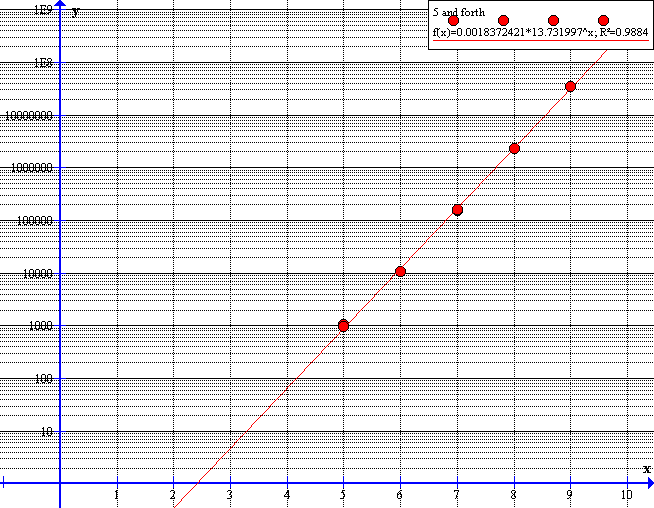
\includegraphics[scale=0.5]{input/pics/timeFunction}
	\caption{\myCaption{The approximation of the time needed to finish the search depth in \m{S} moves. It is displayed on a logarithmic y-axis to show that an exponential function seem to fit.}}
	\label{fig:timeFunction}
\end{figure}

The figure shows the last five data points since the first five are inaccurate due to small amount time which means that other processes might have interfered with the computation time.

As figure \ref{fig:timeFunction} shows the function for approximating the time needed to finish the search depth $x$ is:
\[
f(x)=0.0018372421 \cdot 13.731997^{x} \text{ ms}
\]
The $R^2$ value is close to 1 and this tell us that the approximation is relatively good. The $R^2$ value is a way to express how well a set of data fits onto a specific approximation -- the closer to 1, the better. We are only interested in a rough approximation of how long the solver needs to use to solve a \rubik{}, therefore our $R^2$ value is very acceptable.

We are interested in approximating the time that it would take to solve a \rubik{}. Since the average \rubik{} needs 18 moves to solve \cite{kociemba09} we will estimate the time to compute this:
\[
f(18) = 0.0018372421 \cdot 13.731997^{18} \text{ ms} \approx 5.5383 \cdot 10^{17} \text{ ms} \approx 17600000 \text{ years}
\]

After this time our implementation will have solved an average scrambled \rubik{} with the optimal solution.
However the solver will get into \m{H} a long time before this.
As Michael Reid proved in 1995 \cite{knowledgerush2} it takes a maximum of 12 \twist{}s for Kociemba's optimal solver to enter \m{H}, therefore we have chosen to look at the time it takes for the solver to search inside \m{H} in the second phase.

\subsection{Second Phase}
During our test our solver entered \m{H} many times, all the results are found in appendix \ref{chap:kociembaResults}.
We have chosen to look at the first five times the solver entered \m{H} and make an average from this data.
The reason for the average is that the program which we use to generate the tendency line cannot generate an exponential tendency line from all the data points due to their complexity.

The five runs are shown in table \ref{tab:timeData2}.
\begin{table}[htb]
\centering
	\begin{tabular}{|l|l|l|l|l|l|l|}
	\hline
	Depth& \multicolumn{6}{|c|}{Time to finish [ms]}\\
	\hline
	--&1st time&2nd time&3rd time&4th time&5th time&Average\\
	\hline
	0&0&0&0&0&0&0\\
	\hline
	1&0&0&0&0&0&0\\
	\hline
	2&0&0&0&0&0&0\\
	\hline
	3&0&0&0&0&0&0\\
	\hline
	4&31&0&47&0&0&15.6\\
	\hline
	5&203&62&203&31&47&109.2\\
	\hline
	6&421&374&422&327&328&374.4\\
	\hline
	7&2153&2902&2153&2605&2605&2483.6\\
	\hline
	8&15787&22932&15866&20514&20420&19103.8\\
	\hline
	9&123506&181023&124083&161647&161336&150319\\
	\hline
	10&973348&1430164&977873&1276534&1275302&1186644.2\\
	\hline
	11&7687740&--&7894160&--&--&7790950\\
	\hline
	12&--&--&83980919&--&--&83980919\\
	\hline
	\end{tabular}
\caption{\myCaption{Data for computation time to finish a depth in \m{A} moves of Kociemba's optimal solver in \m{A} moves -- phase two}}
	\label{tab:timeData2}
\end{table}

As with the first phase we assume that an exponential function will make the best approximation to calculate the time spend to finish a given search depth.

\begin{figure}[htb]
	\centering
		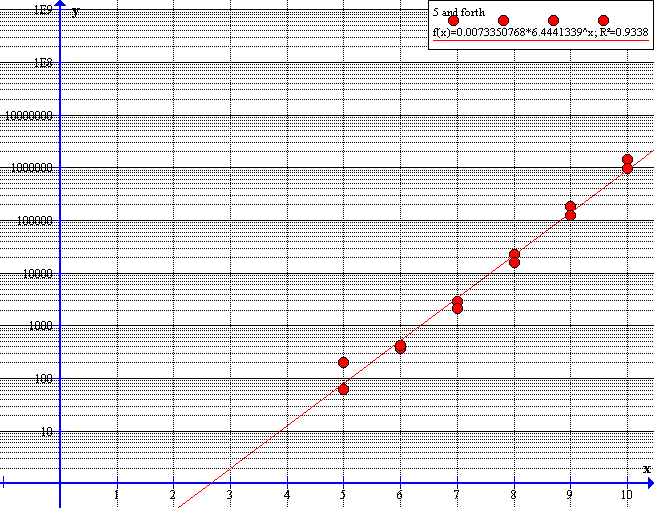
\includegraphics[scale=0.5]{input/pics/timeFunction2}
	\caption{\myCaption{The approximation of the time needed to finish the search depth in \m{A} moves. It is displayed on a logarithmic y-axis to show that an exponential function seem to fit.}}
	\label{fig:timeFunction2}
\end{figure}
Figure \ref{fig:timeFunction2} shows that an exponential function seem to fit quite well due to the relatively high $R^2$ value.
The function to approximate the time need to finish the search depth is seen to be:
\[
f(x) = 0.003438036 \cdot 7.1431204^{x} \text{ ms}
\]
Any \rubik{} that is inside \m{H} can be solve with 18 \m{A} moves.
The time to finish depth 18 will approximately be:
\[
f(18) = 0.003438036 \cdot 7.1431204^{18} \text{ ms} \approx 8.0592 \cdot 10^{12} \text{ ms} \approx 256 \text{ years}
\]